% !TEX TS-program = pdflatexmk
\documentclass[12pt]{amsart}
\usepackage{amsmath}
\usepackage{amssymb}
\usepackage{xcolor}
\definecolor{dark-red}{rgb}{0.7,0.25,0.25}
\definecolor{dark-blue}{rgb}{0.15,0.15,0.55}
\definecolor{medium-blue}{rgb}{0,0,0.65}

\usepackage{tikz}
\usetikzlibrary{cd}
\usetikzlibrary{knots}
\usetikzlibrary{calc}
\usetikzlibrary{matrix}
\usetikzlibrary{arrows,backgrounds,patterns,scopes,external,hobby,
    decorations.pathreplacing,
    decorations.pathmorphing
}
\usepackage{graphicx}
\usepackage{fullpage}
\usepackage[T1]{fontenc}
\usepackage[final]{microtype}
\usepackage{libertine}
\usepackage[libertine]{newtxmath}
\usepackage{ifthen}

\usepackage{pdfpages}

\usepackage[pdftex,plainpages=false,hypertexnames=false,pdfpagelabels,breaklinks]{hyperref}
\hypersetup{
   colorlinks, linkcolor={purple},
   citecolor={medium-blue}, urlcolor={medium-blue}
}
\urlstyle{same}

\newcommand{\mathfig}[2]{{\hspace{-3pt}\begin{array}{c}%
  \raisebox{-2.5pt}{\includegraphics[width=#1\textwidth]{#2}}%
\end{array}\hspace{-3pt}}}

\newcommand{\arxiv}[1]{\href{https://arxiv.org/abs/#1}{\small  arXiv:#1}}

\newcommand{\nn}[1]{{\color{red} [[#1]]}}

% tricky way to iterate macros over a list
\def\semicolon{;}
\def\applytolist#1{
    \expandafter\def\csname multi#1\endcsname##1{
        \def\multiack{##1}\ifx\multiack\semicolon
            \def\next{\relax}
        \else
            \csname #1\endcsname{##1}
            \def\next{\csname multi#1\endcsname}
        \fi
        \next}
    \csname multi#1\endcsname}

% \def\cA{{\cal A}} for A..Z
\def\calc#1{\expandafter\def\csname c#1\endcsname{{\mathcal #1}}}
\applytolist{calc}QWERTYUIOPLKJHGFDSAZXCVBNM;
% \def\bbA{{\mathbb A}} for A..Z
\def\bbc#1{\expandafter\def\csname bb#1\endcsname{{\mathbb #1}}}
\applytolist{bbc}QWERTYUIOPLKJHGFDSAZXCVBNM;
% \def\bfA{{\mathbf A}} for A..Z
\def\bfc#1{\expandafter\def\csname bf#1\endcsname{{\mathbf #1}}}
\applytolist{bfc}QWERTYUIOPLKJHGFDSAZXCVBNM;

\newcommand{\Kar}{\operatorname{Kar}}
\newcommand{\Obj}{\operatorname{Obj}}
\newcommand{\Fun}{\operatorname{Fun}}
\newcommand{\op}{\operatorname{op}}
\newcommand{\Set}{\mathsf{Set}}
\renewcommand{\Vec}{\mathsf{Vec}}
\newcommand{\fdVec}{\mathsf{fdVec}}
\newcommand{\Rep}{\mathsf{Rep}}

\newcommand{\braidcross}{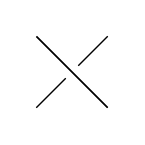
\begin{tikzpicture}[baseline=-0.5ex,scale=0.8]
    \draw (45:.8cm) -- (-135:.8cm);
    \draw[line width=1mm,white,double=black] (-45:.8cm) -- (135:.8cm);
\end{tikzpicture}}
\newcommand{\invbraidcross}{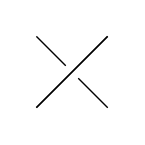
\begin{tikzpicture}[baseline=-0.5ex,scale=0.8]
    \draw (-45:.8cm) -- (135:.8cm);
    \draw[line width=1mm,white,double=black] (45:.8cm) -- (-135:.8cm);
\end{tikzpicture}}
\newcommand{\cupcap}{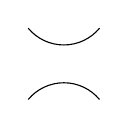
\begin{tikzpicture}[baseline=-0.5ex,scale=0.8]
    \draw (45:.8cm) to [curve through=(90:.3cm)] (135:.8cm);
    \draw (-45:.8cm) to [curve through=(-90:.3cm)] (-135:.8cm);
\end{tikzpicture}}

\newcommand{\twostrandid}{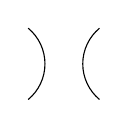
\begin{tikzpicture}[baseline=-0.5ex,rotate=90,scale=0.8]
    \draw (45:.8cm) to [curve through=(90:.3cm)] (135:.8cm);
    \draw (-45:.8cm) to [curve through=(-90:.3cm)] (-135:.8cm);
\end{tikzpicture}}

\begin{document}

\title{Problems for the category theory reading course, 2018}
\author{Scott Morrison}
  \address[Scott Morrison]{
  	Mathematical Sciences Institute,
  	Australian National University
  }
  \email{\href{mailto:scott.morrison@anu.edu.au}{scott.morrison@anu.edu.au}}
\date{Version of \today}

\maketitle 

\section{Assignment 1, due end of Week 3}

\subsection{Functors}
\begin{enumerate}
\item Leinster 1.2.21 (functors preserve isomorphisms)
\item Leinster 1.2.27, 1.2.28b (full, faithful)
\end{enumerate}

\subsection{Natural transformations}
\begin{enumerate}
\item In $\sf{fdVec}$, show that the functors $\operatorname{id}$ and $**$ are naturally isomorphic. 
\item Show the the vertical composition of two natural transformations is in fact a natural transformation. 
\item Prove \emph{carefully} that the horizontal composition of two natural transformations is again a natural transformation.
\item Show that a functor $F : \cC \to \cD$ is part of an equivalence of categories if and only if it is \emph{fully faithful} and \emph{essentially surjective}. (Hint: faithul is easier than full; then use that the inverse of an equivalence is an equivalence.) \footnote{Hint: there's a nice proof in Maclane, or you can try reading \url{https://raw.githubusercontent.com/semorrison/lean-category-theory/master/src/categories/equivalence/characterisation.lean}} \footnote{Did you notice using the axiom of choice?}
\end{enumerate}

\subsection{Universal properties}
\begin{enumerate}
\item Prove that two initial objects in a category are isomorphic.
\item For each of the following categories, decide whether there is an initial, final, and/or zero object, and if so, describe them:
$\sf{FinSet}$, $\sf{fdVec}$, $\sf{Top}$, $\sf{Top}_*$ (pointed topological spaces), $\sf{Semigroups}$, $\sf{Groups}$.
\item Describe the product of two objects as the terminal object in some category.
\item Describe the tensor product of two vectors spaces as the initial object in some category.
\item Describe both the (binary) product and coproduct in the following categories: $\sf{FinSet}$, $\sf{Top}$, $\sf{Top}_*$, $\sf{AbGroup}$, $\sf{Group}$.
\end{enumerate}

\newpage
\section{Assignment 2, due at the end of Week 6}
\subsection{Equivalences}
\begin{enumerate}
\item Choose one of the following pairs of categories, and briefly describe the equivalence (but don't show me all the details -- ideally just talk about the most difficult part):
\begin{itemize}
	\item Compact Hausdorff topological spaces, and commutative $C^*$-algebras.
	\item Subgroups of $\pi_1(X)$, and covers of $X$. (A condition is needed on $X$ to make this work. What is it?)
	\item Subgroups of $\operatorname{Gal}(E \subset F)$, and intermediate field extensions. (A condition is needed on $E \subset F$ to make this work. What is it?)
\end{itemize}
\end{enumerate}

\subsection{Adjunctions}
\begin{enumerate}
\item Consider the forgetful functor from abelian groups to groups. What is its left adjoint?
\item In the category of finite dimensional vector spaces, show that $- \otimes V$ is biadjoint to $- \otimes V^*$.
\item Prove that the `hom-set isomorphism' and `unit/counit' definitions of an adjunction are equivalent.
\end{enumerate}

\subsection{Idempotent completion}
The `idempotent completion' $\Kar(\cC)$ (also called the `Karoubi envelope') is defined as follows:
\begin{align*}
\Obj \Kar(\cC) & = \left\{ (X \in \Obj(\cC), p :  X \to X) \mid| p^2 = p \right\} \\
\Kar(\cC)((X,p) \to (X',p')) & = \left\{ f \in \cC(X \to X') \mid| fp = f = p'f \right\}.
\end{align*}
\begin{enumerate}
\item Let $\mathsf{primeVec}$ denote the full subcategory of $\mathsf{fdVec}$ (the finite dimensional vector spaces) consisting of vector spaces with prime dimensions. Show that $\Kar(\mathsf{primeVec}) \cong \mathsf{Vec}$.
\item Construct an equivalence $\iota_\cC : \Kar(\Kar(\cC)) \cong \Kar(\cC)$.
\item Show that there is a fully faithful functor $\cC \to \Kar(\cC)$ given by $X \mapsto (X, 1_X)$.
\end{enumerate}

\subsection{The Yoneda lemma}
\begin{enumerate}
\item Are there set-theoretic difficulties hiding in the Yoneda lemma?
\item Explain why $\Fun(\cC^\text{op} \to \cD) = \Fun(\cC \to \cD^\text{op})$. Prove that $\Set^\text{op} \ncong \Set$, but that $\fdVec^\text{op} \cong \fdVec$.
\end{enumerate}

\newpage
\section{Assignment 3, due at the end of Week 9}
\begin{enumerate}
% \item Prove that every monoidal category is monoidally equivalent to a strict monoidal category.

% \begin{quote}
% (Hint: given a monoidal category $\cC$, define a new monoidal category $\mathsf{List} \cC$, whose objects are lists of objects in $\cC$. In $\mathsf{List} \cC$, tensor product of objects is concatenation of lists, and the tensor unit is the empty list. There should be a functor $\mathsf{List} \cC$ to $\cC$ defined by sending a list $[x_1, x_2, \ldots, x_n]$ to $(((1 \otimes x_1) \otimes x_2) \otimes \cdots \otimes x_n$. Your job is to describe what happens at the level of morphisms, and check that everything works.)
% \end{quote}

\item Find an example of a monoidal functor which is not naturally isomorphic to any strict monoidal functor.


\begin{quote}
\scriptsize
Hint: consider categories $\Vec^\omega G$, where $G$ is a finite group, and $\omega \in H^3(G, k^\times)$ is a 3-cocycle. In particular, consider $G = \mathbb Z / 2 \mathbb Z$. The category $\Vec \mathbb Z / 2 \mathbb Z$ can be made into a monoidal category in 
a number of different ways. Let's consider the following three associators $\alpha^{(i)}_{X,Y,Z} : (X \otimes Y) \otimes Z \to X \otimes (Y \otimes Z)$. In each case, we'll just say what they do when $X, Y$, and $Z$ are 1-dimensional vector spaces (so either $\mathbb C_{\text{even}}$, in the even grading, or $\mathbb C_{\text{odd}}$, in the odd grading).
\begin{align*}
\alpha^{(1)}_{X,Y,Z} & = 1 \\
\alpha^{(2)}_{X,Y,Z} & = \begin{cases} 1 & \text{if $Z = \mathbb C_{\text{even}}$} \\ -1 & \text{if $Z = \mathbb C_{\text{odd}}$} \end{cases} \\
\alpha^{(3)}_{X,Y,Z} & = \begin{cases} 1 & \text{if any of $X, Y$, or $Z$ are $\mathbb C_{\text{even}}$} \\ -1 & \text{if all if $X, Y$, and $Z$ are $\mathbb C_{\text{odd}}$} \end{cases}
\end{align*}
If you're going to use this example you should explain carefully why these are actually associators. You should be able to show that there are 
no monoidal functors, strict or otherwise, from $(\Vec \mathbb Z / 2 \mathbb Z, \alpha^{(3)})$ to $(\Vec \mathbb Z / 2 \mathbb Z, \alpha^{(1)})$, and moreover
that there are monoidal functors, but no strict ones, from $(\Vec \mathbb Z / 2 \mathbb Z, \alpha^{(2)})$ to $(\Vec \mathbb Z / 2 \mathbb Z, \alpha^{(1)})$.
You should be able to explicitly write down such functors, with tensorators.

To make sure you really know what's going on, you might think about these questsions:
\begin{itemize}
\item What about functors back the other way?
\item Which of these categories are equivalent?
\item What are all the associators on $\Vec \mathbb Z / 2 \mathbb Z$?
\item Which of these associators give categories that are monoidally equivalent to each other?
\end{itemize}
\end{quote}

\item Let $\cC$ be a monoidal category. We say a `monoid object' in $\cC$ (or, as we gain confidence, just a monoid in $\cC$) is a tuple $(A \in \Obj C, \iota: 1 \to A, m: A \otimes A \to A)$ satisfying some conditions. Look up, or work out, what these conditions should be. (Hint: look at chapter 7 of Etingof, Gelaki, Nikshych, and Ostrik's book \href{http://www-math.mit.edu/~etingof/egnobookfinal.pdf}{Tensor Categories}.) You should be able to show that a monoid object in $\mathsf{Vec}$ is what is usually called an associative unital algebra.

A `module object' for a monoid object $A \in \cC$ is a tuple $(M, \triangleright: A \otimes M \to M)$ satisfying an appropriate condition. A morphism $f$ between module objects $M$ and $M'$ is a morphism between the underlying objects, such that $f \circ \triangleright_M = \triangleright_{M'} \circ (1_A \otimes f)$.
\begin{enumerate}
\item What is the complete definition of a module object?
\item Draw the string diagram corresponding to the axiom describing module object morphisms.
\item Define composition of module morphisms, by imitating the definition for modules over a ring.
\item Show that modules for a fixed monoid object form a category.
\end{enumerate}
\item Show that $\Rep G$, for $G$ a finite group, forms a monoidal category.
\item (For this part, you may assume we are looking at representations over the complex numbers, and $G$ and $H$ are finite.)
\begin{itemize}
\item If $\Rep G \cong \Rep H$, as categories, are $G$ and $H$ isomorphic?
\begin{quote}
\scriptsize
Hint: no, give a counterexample --- any pair of non-isomorphic groups with the same number of irreducible representations (equivalently, the same number of conjugacy classes) will do.
\end{quote}
\item
What about if $\Rep G \cong \Rep H$ as monoidal categories, and moreover this equivalence is compatible with the forgetful functors to $\Vec$?
\begin{quote}
\scriptsize

Hint: think about the monoidal automorphisms of the forgetful functor. You should prove that (not necessarily monoidal) automorphisms of the forgetful functor $\Rep G \to \Vec$ is a group isomorphic to $\mathbb C[G]^{\times}$, and then identify that the subgroup of monoidal automorphisms is $G$ itself. To do the first part, show that any such automorphism is determined by its component on the regular representation $\mathbb C[G]$; for this you may like to use that the regular representation is faithful, or (more or less equivalently) that there is a surjective $G$-linear map from the regular representation to any irreducible representation of $G$.
\end{quote}
%\item What if we drop the condition about compatibility with the forgetful functors? (Hint: google `isocategorical group'; you can answer this with just an appropriate reference to the literature, or do it yourself.)
\end{itemize}
\end{enumerate}


\newpage
\section{Assignment 4, due at the end of Week 12}

\subsection{Braided monoidal categories}
\begin{enumerate}
\item Show that Temperley-Lieb is a braided monoidal category, with braiding satisfying
$$\braidcross =  A \twostrandid + A^{-1} \cupcap,$$
for some $A$ so that $\delta = -A^2 - A^{-2}$.
\item
We can take a link diagram, and interpret it as a morphism $0 \to 0$ in Temperley-Lieb, by interpreting crossings according to the above formula. (Explain carefully what we're meant to do with \scalebox{0.5}{$\invbraidcross$}.)
The morphism space $0 \to 0$ consists of just scalar multiples of the empty diagram, so this associates a number to a link diagram. Explain why this number is a \emph{framed} link invariant, i.e. that it doesn't change when we modify the link diagram by Reidemeister moves II and III, and a \href{https://en.wikipedia.org/wiki/Reidemeister_move}{modified} version of the usual Reidemeister move I.
\item Calculate the invariant of the trefoil, according to this recipe. Show that the trefoil is not isotopic to the unknot, by showing this invariant takes different values on the two knots.
\item What is this invariant usually called?
\item Show that in $\Kar(TL)$, we have $(2,1_2) \cong (2,f^{(2)}) \oplus (0, 1_0)$. Here $f^{(2)}$ denotes the second Jones-Wenzl idempotent:
$$f^{(2)} = \twostrandid -\frac{1}{\delta} \cupcap
.$$
\item 
We can make another knot invariant by replacing each string of a knot diagram by two parallel strings, and somewhere on the knot inserting a copy of $f^{(2)}$.
$$\mathfig{0.2}{cabled-trefoil}$$
Explain why this doesn't depend on where we insert the $f^{(2)}$. Calculate this invariant for the unknot.
\item We say a monoid $(A, m)$ in a braided monoidal category is commutative if $m \circ \beta = m$, where $\beta$ denotes the braiding. Define a monoidal structure on the category of comodules for a commutative monoid.
\end{enumerate}


\end{document}

\newpage
\subsection{Abelian categories}
\begin{enumerate}
\item Show that in a rigid abelian category, the functor $- \otimes X$ is exact. (Proposition 2.1.8 of Bakalov-Kirillov, attached,
gives a terse proof of this. I'd like you to carefully explain their steps. You may find the discussion at \url{https://math.stackexchange.com/q/98877/} helpful.)
\end{enumerate}


\section{Odds and ends}
\subsection{More on adjoints}
\begin{enumerate}  
\item* Consider the forgetful functor from compact Hausdorff spaces into Hausdorff spaces. Show that its left adjoint is Stone-\v{C}ech compactification.
\item Recall the $\cC-\mathsf{Set}$ is the category of functors from $\cC$ to $\mathsf{Set}$. Given a functor $F : \cC \to \cD$, we have the pull-back functor $F^* : \cD-\mathsf{Set} \to \cC-\mathsf{Set}$ given by precomposition by $F$. If $F^*$ has adjoints, we call them the right push-forward $F_*$ and the left pushforward $F_!$ (pronounced usually `$F$-shriek').

(You may like to read \url{https://arxiv.org/abs/1009.1166}.)
\begin{enumerate}
	\item \nn{Calculate some examples.}
	\item Show that the polynomial functors, namely those of the form $F_! G^* H_* : \cE-\mathsf{Set} \to \cB-\mathsf{Set}$ for some diagram $$\cB \xleftarrow{F} \cC \xrightarrow{G} \cD \xleftarrow{H} \cE,$$ are closed under composition. (You may assume that all categories are finitely presented, i.e. the path category of some finite graph modulo finitely many relations. You may like to look at \url{https://ncatlab.org/nlab/show/polynomial+functor}, although as is often the case at the \emph{nLab}, the presentation there is more general than we need.) 
\end{enumerate}

\end{enumerate}



\end{document}

